\documentclass[preprint,number,12pt]{elsarticle}

%% Language and font encodings
\usepackage[english]{babel}
\usepackage[utf8x]{inputenc}
\usepackage[T1]{fontenc}

%% Sets page size and margins
\usepackage[left=4cm,right=4cm,marginparwidth=3cm]{geometry}

%% Useful packages
\usepackage{amsmath}
\usepackage{amsthm}
\usepackage{amssymb}
\usepackage{bm}
\usepackage{graphicx}
\usepackage{lineno}
\usepackage[ruled,vlined]{algorithm2e}
%\usepackage{natbib}

\usepackage[colorinlistoftodos,textsize=tiny]{todonotes}
\usepackage[colorlinks=true, allcolors=blue]{hyperref}

\newtheorem{theorem}{Theorem}[section]
\newtheorem{corollary}{Corollary}[theorem]
\newtheorem{lemma}[theorem]{Lemma}

\biboptions{comma,square,numbers}

\journal{bioRxiv}

\begin{document}

\begin{frontmatter}
\title{Streaming Construction of the Compact de Bruijn Graph}

\author[ggcs]{C. S. Welcher}
\ead{cswel@ucdavis.edu}

\author[pop,ggcs]{C. Titus Brown}
\ead{ctbrown@ucdavis.edu}

\address[ggcs]{Graduate Group for Computer Science, University of California, Davis}
\address[pop]{Department of Population Health and Reproduction, School of Veterinary Medicine, University of California, Davis}

\begin{abstract}
The widespread adaptation and growth in sequencing technologies has demanded parallel advancement in  computational methods for sequence analysis. In sequence assembly, the assembly graph has become ubiquitous as an abstraction for both encoding and analyzing the results of sequencing experiments.
\todo[inline]{Camille: complete abstract.}
\end{abstract}

\end{frontmatter}


\linenumbers
\section{Background}

\subsection{Context}\label{sec:context}

Developments in high-throughput sequencing technology over the past two decades have made genomics, transcriptomics, metagenomics, and their variants core methods in biological inquiry.
De novo assembly converts a set of fragments produced from one of these methods into an approximation of the underlying sampled sequence.
While early methods directly computed overlaps between shallowly-sampled fragments \cite{roach_random_1995}, deep sequencing has led to the use of assembly graphs as the core abstraction in assembly \cite{myers_toward_1995,simpson_theory_2015,chikhi2016compacting}.
The de Bruijn graph \cite{myers_fragment_2005,li_exploring_2012,zerbino_velvet:_2008,pevzner2001eulerian} remains one of the core assembly graph constructions for short reads, and its $k$-mer based approach finds utility for long read technology as well\todo{Camille: citations to minimap, minhash, pathset graphs}.
In the de Bruijn Graph, sequences are broken down into subsequences of length $k$, or $k$-mers, with edges between $k$-mers with prefix-suffix overlaps of length $k-1$; this implicit definition of edges obviates the need for explicit overlap computation, making de Bruijn Graphs well-suited to ultra-deep sequence experiments with short reads (see \ref{sec:definitions}).
While this property greatly improves the time scaling of the assembly problem, the de Bruijn Graph suffers from extremely high storage requirements due to the enumeration of $k$-mers.
To address this, it is often compacted by the contraction of linear paths of non-branching $k$-mers, forming the compact de Bruin Graph.

A number of approaches for generating the compact de Bruijn Graph are already established. BCALM 2 generates a compact de Bruijn Graph in parallel using ranked minimizers \cite{chikhi2016compacting}, building on their previous work on de Bruijn graph representation in general \cite{chikhi2015representation}.
Velvet \cite{zerbino_velvet:_2008} and Trinity \cite{grabherr_full-length_2011} generate compact de Bruijn Graphs in intermediate steps.
Regardless of the method for generating the graph, almost all extant approaches share a paradigm: they are off-line algorithms, algorithms which require access to the entire sample before proceeding with compaction, and possibly make multiple passes over the data.
In contrast, streaming (or online) algorithms view their data as a stream of observations, and make one or fewer passes over that stream \cite{mcgregor_graph_2014}, while semi-streaming algorithms aim for a small, constant number of passes, generally two or fewer \cite{feigenbaum_graph_2005}.
Streaming approaches have several advantages: they minimize hard disk access, which aids in efficiency; they are often able to produce results opportunistically, as soon as they are available; they offer the potential for feedback between the data stream and the processing; and often, they are suited for handling streams of infinite length\todo{Camille: This might be a good place to mention the accessibility component as well: reducing download requirements for labs with limited resources and internet access.}.

\todo[inline]{Camille: Bring in overview of streaming paradigm in bioinformatics. My proposal has a good start, but there are others I've missed.}

Here, we explore an implementation of a streaming de Bruijn graph compactor. Our implementation builds the compact de Bruijn graph opportunistically from a stream of sequence fragments, in one pass over the data. While a semi-streaming de Bruijn graph compactor has been previously published \textbf{[cite Faucet]}, this is to our knowledge the first implementation of a streaming compact de Bruijn graph.

\subsection{Definitions}\label{sec:definitions}

For this section, let $S[i]$ represent the symbol at position $i$ for some string $S$, $0$-indexed, and $S[i:j]$ be the substring of $S$ starting at position $i$ and not including position $j$. 
If $S$ has length $L$, the $k$-mers of $S$ are given by $\texttt{kmers}(S) = \{S[i:i+k] \mid 0 \le i < L-k+1 \}$ ; that is, all length $k$ substrings of $S$.
When $S$ is over the alphabet $\Sigma=\{A,C,G,T\})$, we call $S$ a nucleotide sequence, or sequence; for the remainder of this paper we assume this alphabet.
Additionally, for a $k$-mer $u$, let $\texttt{pre}(u)=u[0:k-1]$ and $\texttt{suf}(u)=u[1:k]$. 
For a de Bruijn graph $G_{k, \Sigma} = (N,E)$, $N$ is a set of $k$-mers over alphabet $\Sigma$, and $E$ is the set of length $K$-1 suffix-prefix overlaps between $k$-mers in $N$; that is, $E = \{e_{u \rightarrow v} \mid \texttt{suf}(u) = \texttt{pre}(v) \forall u,v \in N \}$.

Given a set of sequences $SS$, the de Bruijn graph $G_k(SS)$  has $N = \bigcup_{s \in SS}{\texttt{kmers}(s)}$.
Note that our edge definition admits edges even when the corresponding ($k+1$)-mers containing the two overlapping $k$-mers are not present in any sequence in $SS$; this is the node-centric de Bruijn graph, and edges are defined implicitly, rather than explicitly encoded.
If we define $\texttt{query}(u, G_k) = \begin{cases} 1 & u \in N \\0 & u \notin N \end{cases}$, we can then discover the right-neighbors (those with $u$ as in in-edge) of $u$ with the function $\texttt{rneighbors}(u, G_k) = \{\texttt{query}(\texttt{suf}(u) + c), G_k) \forall c \in \Sigma\}$, and the left-neighbors (those with $u$ as an out-edge) with $\texttt{lneighbors}(u, G_k) = \{\texttt{query}(c + \texttt{pre}(u), G_k) \forall c \in \Sigma\}$.

Now let $SS$ be an ordered stream of sequences rather than a set. $SS[t]$ is then the $t$th sequence in the stream, indexed in the same manner as our strings, and $G_k(SS)[t]$ is the de Bruijn graph with $N = \bigcup_{s \in SS[0:t+1]}{\texttt{kmers}(s)}$.
The total number of sequences in $SS$ may or may not be known. We refer to the position $t$ in the stream as the $time$.
$time$ may be analogous to actual observation time or simply position within a file, depending on the source of the stream.

The compact de Bruijn graph (cDBG) is built from the  de Bruijn graph by converting non-branching paths of $k$-mers into single nodes.
Define $C(G_k) = (N_c, E_c)$ as the compact de Bruijn graph built from $G_k$; for brevity, we call it $C_k$.
A node $u \in G_k$ is a \textit{decision node} if $|\texttt{rneighbors}(u, G_k)| = 1$ or $|\texttt{lneighbors}(u, G_k)| > 1$.
$N_d$ is the complete set of decision nodes in $G_k$.
Consider a connected path $p = \{u_0, u_1, ... , u_L\} \in G_k$, where $L$ is the number of nodes in $p$. $p$ is a unitig if none of $u_1 ... u_{L-1}$ are decision nodes, and $p$ cannot be further extended in either direction.
The complete set of unitigs will be called $U$, and we define $N_c = N_d \cup U$.
We add edges to $E_c$ when a node in $N_d$ matches the first or last node in a unitig from $U$. Let $d_i \in N_d$ and $u_i \in U$; then any path in $C_k$ must take the form $\{u_i, d_i, u_{i+1}, d_{i+1}, ...\}$; that is, unitig nodes may never be neighbors, and unitig nodes will have both in-degree and out-degree of at most one.

\begin{figure}
	\centering
	\missingfigure[figwidth=\textwidth]{Paneled figure showing the raw de Bruijn graph structure, the cDBG structure, and the relationship between the two.}
	\caption{\label{fig:cdbg-structure}a)  The underlying de Bruijn graph. Decision nodes are colored red. 
		b) The \texttt{boink} compact de Bruijn graph model. Decision nodes are shared with the underlying de Bruijng graph, and unitig nodes are mapped back to minimizers of their corresponding unitig paths. }
\end{figure}

A unitig node with no neighboring decision nodes is an $island$; a unitig node with decision nodes on either side is $full$; and a unitig node with a decision node on only one side is a $tip$. As with the de Bruijn graph, we refer to the cDBG at time $t$ as $C_k[t]$.

\todo{Camille: Give definition of tagging and minimizers.}

\section{Methods}\label{sec:methods}

The streaming de Bruijn graph compactor is implemented in the \texttt{boink} \cite{boink} package hosted on GitHub, and links against \texttt{khmer} \cite{crusoe2015khmer} for sequence parsing and $k$-mer counting. 
Core functionality is implemented in C++ and wrapped in Cython to provide a Python interface; high-level scripts and analyses are implemented in Python.

Broadly, the underlying de Bruijn graph is implemented as a set with a probabilistic data structure. Sequences are broken down into constituent $k$-mers and hashed, and if a sequence contains any $k$-mers not previously observed in the de Bruijn graph, the cDBG is updated from the sequence. A subset of $k$-mers $T$ in the de Bruijn graph are "tagged" using a random minimizer scheme \cite{roberts2004reducing,marccais2017improving}; these $k$-mers are used to map from the de Bruijn graph to unitig nodes in the cDBG. The neighborhood of the new sequence is searched for decision nodes that could be disturbed by adding it, and unitig nodes that intersect its new $k$-mers. cDBG operations are placed on a work queue, where they are processed by a separate thread what manages updates to the cDBG.

The next sections describe the compaction process and implementation in detail.

\subsection{Construction of the de Bruijn Graph}\label{sec:dbg-construction}

The de Bruijn graph is implemented as a simple set of $k$-mers.
As such, it can be updated in a streaming fashion with no additional methods: a new sequence $s_t$ from $SS$ is broken down into its constituent $k$-mers and hashed with an efficient rolling hash scheme \cite{lemire2010recursive}, with new $k$-mers being added to the set and existing $k$-mers being incremented if a counting data structure is in use.
The use of a node-centric de Bruijn graph model helps with this step, removing the need for any traversal to find neighbors of new $k$-mers or the explicit encoding of edges.

The de Bruijn graph uses a probabilistic data structures from the \texttt{khmer} \cite{crusoe2015khmer,pell_scaling_2012} package, which support low-memory use at the cost of a small false-positive rate, for storing $k$-mers. Currently supported data structures for $k$-mer storage are Bloom filters \cite{bloom_space/time_1970}, Count-Min Sketches, the Counting Quotient Filter \cite{cqf2017}, and an efficient exact hash-set using Sparseppp (github.com/greg7mdp/sparsepp), which is based on Google's sparsehash. 
It was previously shown that false positives have minimal effect on the global structure of the de Bruijn graph when under $\sim0.17$ \cite{pell_scaling_2012}; however, to avoid accumulation of many false tips and decision nodes in the cDBG by false positives neighboring true positives, this should be kept as low as possible \cite{chikhi_space-efficient_2013}.

\subsection{cDBG Data Structure}\label{sec:cdbg-data-structure}

The cDBG data structure consists of two maps: first, a basic hash table of known decision nodes $N_d$, and a map from $k$-mer hashes of the ends of unitig paths to the unitig nodes $U$. These two structures are sufficient to define the entire cDBG: neighbors of decision nodes are necessarily tips in $U$, and island unitigs can be discovered from their tips. However, in order to split existing unitigs, potentially long traversals would need to be made from induced decision $k$-mers to unitig ends; as such, we store an auxiliary map $T$ from the minimizers of the unitig paths to the unitigs. This sets the maximum traversal distance from an induced decision $k$-mer to find the unitig containing it to the window size $w$ of the minimizer.

\subsection{Mutations to the cDBG}\label{sec:cdbg-mutations}

The streaming compact de Bruijn graph can be defined by its decision $k$-mers and the $k$-mers terminating its current unitigs. While unitigs are subject to mutation throughout streaming construction (splitting and merging), decision nodes within the cDBG are never deleted once created, a property which can be exploited for construction (CTB: during graph construction?).

First, let us define the essential mutations on the streaming cDBG. A \textit{new} $k$-mer in $G_t$ is a $k$-mer not present in $G_{t-1}$; that is, a $k$-mer first introduced in fragment $t$. A \textit{new decision $k$-mer} is a new $k$-mer which is also a decision $k$-mer. An \textit{induced decision $k$-mer} is a decision $k$-mer which is not new, but became a decision $k$-mer at time $t$. A \textit{new unitig node} is a unitig comprising only new $k$-mers. An existing unitig node is \textit{split} when one its $k$-mers becomes an induced decision $k$-mer, and two unitig nodes are merged when a path of new $k$-mers exists between two of their tip $k$-mers. Given a sequence $s_t \in SS$, the \textit{segments} of $s_t$ are the paths of new $k$-mers in $s_t$, split at existing $k$-mers and new decision $k$-mers. Now, we will define the ways in which a segment can mutate the cDBG.

\subsubsection{Inserting New Sequences and Finding New Segments}\label{sec:insertion}

The first step to updating the cDBG with a new sequence is to insert its $k$-mers into the dBG and divide its new $k$-mers into their constituent segments. Once we have the segments, we use them to update the state of the cDBG. \ref{FindSegments} describes this procedure: segment paths are split on existing $k$-mers and new decision $k$-mers.

\begin{algorithm}[]
	\DontPrintSemicolon
	\KwData{dBG $G_{k,t-1}$, sequence stream $SS$}
	\KwIn{sequence $s_t \in SS$ }
	\KwResult{A list $\ell$ of new segments from $s_t$, set of new decision $k$-mers $\delta$}
	$U \longleftarrow kmers(s_t)$\;
	$P \longleftarrow \emptyset$\;
	\For{$u \in U$}{
		$P.append(G.query(u))$\;
		$G.insert(u)$\;
	}
	$p \longleftarrow \bm{False}$\;
	$v \longleftarrow U[0]$\;
	$segment \longleftarrow \emptyset$\;
	\For{$v \in U$, $q \in P$}{
		\If{$q = \bm{True}$}{
		
			\If{$p \not= \bm{False}$}{
				$segment \longleftarrow \{u\}$
			}
			\If{$G.lneighbors(v) > 1 \parallel G.rneighbors(v) > 1$}{
				\If{$v \not= U[0]$}{
					$\ell.append(segment)$
				}
				$segment \longleftarrow \{v\}$\;
				$\delta.insert(v)$\;
			}
		}\ElseIf{$p = \bm{True}$}{
			$\ell.append(segment)$\;
			$segment \longleftarrow \emptyset$\;
		}
	
		$u \longleftarrow v$\;
		$p \longleftarrow q$\;
	}
	\If{$q = \bm{True}$}{
		$\ell.append(segment)$
	}
	\Return{$\ell, \delta$}
\caption{FindSegments\label{FindSegments}}
\end{algorithm}

Only certain $k$-mers are able to induce an existing $k$-mer to become a decision $k$-mer, and thereby potentially split an existing unitig. \ref{InduceDecisionKmers} lays out the procedure for handling these $k$-mers, which can be only the first or last $k$-mer in a segment or a new decision $k$-mer; see \ref{inducers-lemma}.

\begin{algorithm}
	\DontPrintSemicolon
	\KwData{dBG $G_{k,t-1}$, cDBG $C(G_{k,t-1})$}
	\KwIn{$k$-mer $u$ which can induce decision $k$-mers, set $\Delta$ of new $k$-mers to ignore }
	\For{$v \in G.neighbors(u)$}{
		\If{$v \notin \Delta$ and $IsDecision(v)$}{
			$C.NewDecisionNode(v)$\;
			$C.SplitUnitig(v)$\;
		}
	}
\caption{InduceDecisionKmers}\label{InduceDecisionKmers}
\end{algorithm}

With this procedure defined, we are able to update the cDBG from the new segment. We attempt to induce decision $k$-mers from the first and last $k$-mers in the segment and split unitigs if necessary; if the first or last $k$-mer is not a new decision $k$-mer and does not match up to an existing unitig tip \ref{tip-corollary}, we search for induced decision $k$-mers only in the direction away from the segment.
\todo[inline]{Camille: Write corollary showing we only need the one direction... update implementation for this!}
If neither end of the segment matches to an existing unitig, we produce a new unitig with just the segment. The full procedure is detailed in \ref{InsertSegment}.

\begin{algorithm}
	\DontPrintSemicolon
	\KwData{dBG $G_{k,t-1}$, cDBG $C(G_{k,t-1})$}
	\KwIn{list of $k$-mers comprising $segment$ from $s_t \in SS$, 
			 set of new decision $k$-mers $\delta$,
		 	 set of all new $k$-mers $\Delta$}
	 
	 $l, r \longleftarrow \bm{True}$\;
	\If{$segment.first \in \delta$}{
		$C.NewDecisionNode(segment.first)$\;
		$InduceDecisionKmers(segment.first, \Delta)$\;
	} \ElseIf{$G.lneighbors(segment.first) \notin C.U$} {
		$InduceLeftDecisionKmers(segment.first, \Delta)$
	} \Else{
		$l \longleftarrow \bm{False}$\;
		$C.ExtendUnitig(G.lneighbors(segment.first), segment)$\;
	}

	\If{$segment.last \in \delta$}{
		$C.NewDecisionNode(segment.last)$\;
		$InduceDecisionKmers(segment.last, \Delta)$\;
	} \ElseIf{$.rneighbors(segmen.last) \notin C.U$ } {
		$InduceRightDecisionKmers(segment.last, \Delta)$
	} \Else {
	    $r \longleftarrow \bm{False}$\;
		$C.ExtendUnitig(G.rneighbors(segment.last), segment)$\;
	}

	\If{$l = r = \bm{True}$}{
		$C.NewUnitig(segment)$
	}
\caption{InsertSegment}\label{InsertSegment}
\end{algorithm}

\subsubsection{Splitting Existing Unitigs from Induced Decision $k$-mers}\label{sec:splitting}

\begin{enumerate}
	\item Description of tagging: the minimizers and linking between unitig nodes and tags. References 
	\item Untig spliting process: searching for minimizers and performing split
	\item There should be a corollary that there are exactly two directions to search for tags and thereby exactly one unitig to split
\end{enumerate}

\subsubsection{Correctness}\label{sec:correctness}

\begin{lemma}[inducers-lemma]
	\label{inducers-lemma}
	A decision $k$-mer can only be induced by a new decision $k$-mer in $s_t$ or the first or last $k$-mers in a new segment of $s_t$.
\end{lemma}

\begin{proof}
	Consider an existing non-decision $k$-mer $\mu \notin s_t$. An existing $k$-mer in $s_t$ cannot induce $\mu$ to be a decision $k$-mer: if so, $\mu$ would already be a decision $k$-mer. Now consider a new $k$-mer $\nu$ in the fragment which is not the first or last $k$-mer of a segment. In order for $\nu$ to induce $\mu$ to be a decision $k$-mer, $\mu$ must be a neighbor of $\nu$; because $\nu$ is not an end $k$-mer, it already has in-degree and out-degree at least one, from the new $k$-mers on either side of it. Now consider an end $k$-mer of a new segment: it has at least one new $k$-mer as its neighbor, and possibly an existing $k$-mer $\mu$ as its other neighbor. If $\mu$ is an in-neighbor of $\nu$, and already has out-degree of one, then $\nu$ can induce $\mu$ while being a non-decision $k$-mer; this exists for the case where $\mu$ is an out-neighbor as well.
\end{proof}

\begin{lemma}[splitting-lemma]
	\label{splitting-lemma}
	An existing unitig node can only be split by an induced decision $k$-mer.
\end{lemma}

\begin{proof}
	An existing unitig is, by definition, composed of existing non-decision $k$-mers. A new $k$-mer cannot split an existing unitig, also by definition: if the $k$-mer were part of the unitig, it would not be new. Thus, in order to split a unitig, we must convert an existing $k$-mer into a decision $k$-mer. 
\end{proof}

\begin{corollary}
	\label{tip-corollary}
	If a $k$-mer $\mu$ which is the first or last $k$-mer of a new segment has a neighbor $\nu$ which is not a unitig tip, then $\nu$ must be an induced decision $k$-mer.
\end{corollary}



\begin{figure}
	\centering
	\missingfigure[figwidth=\textwidth]{Figure illustrated disturbed decision nodes.}
	\caption{\label{fig:disturbed-dnodes}Caption describing decision nodes, references algorithm.}
\end{figure}

\subsection{Asynchronous Operations}\label{sec:async}

\todo[inline]{Camille: Not sure if this section is relevant or necessary beyond my thinking it's cool.}

\texttt{boink} uses an event-listener model common in systems design to support asynchronous operations for parsing, de Bruijn graph construction, cDBG updates, and statistical output.
Objects can be either Listeners or Notifiers. A Listener consists of a queue protected by a mutex, a set of event types to listen for, a public function to add events to the queue, and a worker thread to process events from the queue when available. A Notifier keeps a list of references to Listeners, and exposes a public method for listeners top register themselves. When the notifier calls its notify method, all registered Listeners are notified of the event. For example, a parsing object is implemented as a Notifier, which processes the sequence stream and calls the update methods on the compactor. At set intervals, it notifies its listeners that some time interval has been reached; functionality for computing various statistics on the cDBG implement Listeners which output their computations at their appropriate intervals. This allows operations requiring slow disk access to lag behind the compactor. Similarly, the cDBG itself is a Listener registered on the compactor; traversals on the de Bruijn graph can then proceed while the cDBG is updated off its event queue. This model offers substantial improvements both in speed and conceptual clarity.

\section{Results}\label{sec:results}

\subsection{Streaming cDBG Construction Produces Correct Results in Reasonable Time}\label{sec:correctness}

This section should include a description of the validation pipeline and some benchmarks. The goal here is not to show that \texttt{boink} is the fasted raddest compactor around, but rather that it works and can be used on real data. I'm holding off on benchmarking until I've completing some additional performance improvements, as I want performance to not be entirely horrible.

\subsection{Streaming Methods Yield New Approaches for Studying Sequence Data and Assembly Graphs}\label{sec:approaches}

\begin{figure}
	\centering
	\missingfigure[figwidth=\textwidth]{Assembly graph growth on exemplar data.}
	\caption{\label{fig:exemplars}A figure with unit-scaled growth for a transcriptome, a genome, and a metagenome; or possibly, average trendlines for a few of each. I think a better metric for global structure should be used here: either Laplacian spectrum, or graphlet kernel spectrum.}
\end{figure}

Explore assembly graph statistics for txomes, genomes, and metagenomes. Idea is to briefly describe general trends in assembly graph growth for different data types. This also illustrates that the approach can scale.

\todo{Camille: Choose an exemplar transcriptome / set of transcriptomes. Probably an MMETSP sample, a vertebrate sample, and some noisy sample (lamprey?).}
\todo{Camille: Choose an exemplar genome / genomes.}
\todo{Camille: Choose an exemplar metageome. Probably one mock community and one reasonably-sized wild community.}

\subsection{An Analysis of Sequence Artifacts Through Streaming cDBG Construction}\label{sec:artifacts}

Here, I'll explore the MMETSP sequencing artifacts.

The first plot will be showing two MMETSP samples, one with minimal artifacts and one with large aberrations. Open question whether this is a worthwhile section, but I think showing a real world use case is useful. An alternative real-world use-case is a streamed download producing a cDBG; but, an interesting biological use-case makes the paper more interesting to a wider audience, in my opinion.

\begin{figure}
\centering
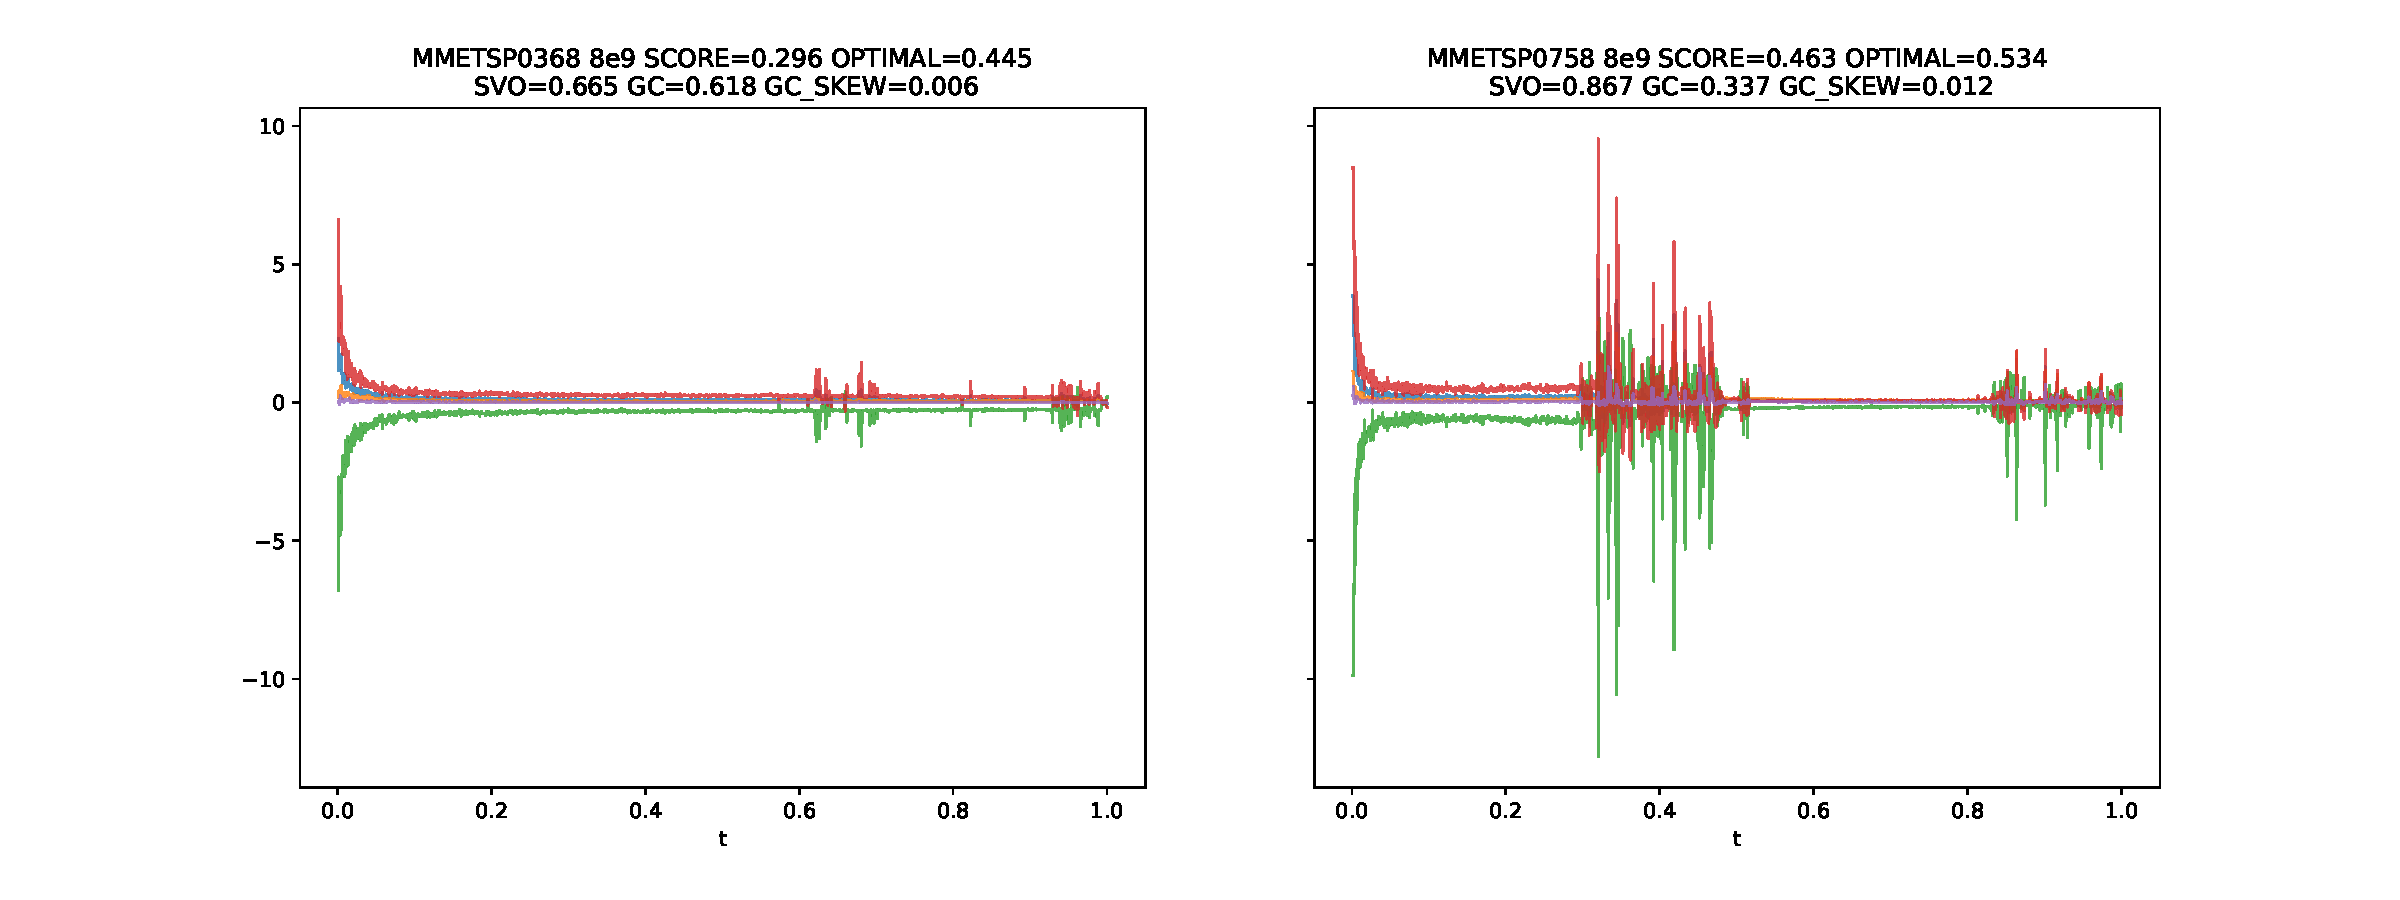
\includegraphics[width=\textwidth]{figures/mmetsp_artifacts}
\caption{\label{fig:artifacts}An example of artifactual samples. The sample on the left displays minimal non-randomness; the sample on the right displays extreme artifacts throughout the file.}
\end{figure}

\section{Conclusions}\label{sec:conclusions}

\begin{enumerate}
	\item Streaming algorithms are practically useful.
	\item Streaming analysis of assembly graphs provides new insights into their structure.
	\item Future applications for real-time long read technology.
	\item Discussion of accessibility.
\end{enumerate}

\bibliographystyle{tex/model1-num-names}
\bibliography{tex/streaming}

\listoftodos

\end{document}
